%
% File eacl2017.tex
%
%% Based on the style files for ACL-2016
%% Based on the style files for ACL-2015, with some improvements
%%  taken from the NAACL-2016 style
%% Based on the style files for ACL-2014, which were, in turn,
%% Based on the style files for ACL-2013, which were, in turn,
%% Based on the style files for ACL-2012, which were, in turn,
%% based on the style files for ACL-2011, which were, in turn, 
%% based on the style files for ACL-2010, which were, in turn, 
%% based on the style files for ACL-IJCNLP-2009, which were, in turn,
%% based on the style files for EACL-2009 and IJCNLP-2008...

%% Based on the style files for EACL 2006 by 
%%e.agirre@ehu.es or Sergi.Balari@uab.es
%% and that of ACL 08 by Joakim Nivre and Noah Smith

\documentclass[11pt]{article}
\usepackage{eacl2017}
\usepackage{times}
\usepackage{url}
\usepackage{latexsym}
\usepackage{natbib}
\usepackage{amsmath}
\usepackage{subfigure}
\usepackage{graphicx}

% \eaclfinalcopy % Uncomment this line for the final submission
%\def\eaclpaperid{***} %  Enter the acl Paper ID here

%\setlength\titlebox{5cm}
% You can expand the titlebox if you need extra space
% to show all the authors. Please do not make the titlebox
% smaller than 5cm (the original size); we will check this
% in the camera-ready version and ask you to change it back.

\newcommand\BibTeX{B{\sc ib}\TeX}

\title{Learning to Negate Adjectives with Bilinear Models}
% Learning to Negate Adjectives with Relational Antonym Encoders
% Learning to Negate Adjectives with Continuous Class-Conditional Relational Encoders

\author{First Author \\
  Affiliation / Address line 1 \\
  Affiliation / Address line 2 \\
  Affiliation / Address line 3 \\
  {\tt email@domain} \\\And
  Second Author \\
  Affiliation / Address line 1 \\
  Affiliation / Address line 2 \\
  Affiliation / Address line 3 \\
  {\tt email@domain} \\}

\date{}

\begin{document}
\maketitle
\begin{abstract}
 TODO
\vspace{15mm}
\end{abstract}

\section{Introduction}

Identifying antonyms in a vector space model is a notoriously
challenging task, because the vectors for related words of opposite
polarity, such as {\it hot} and {\it cold}, are close to each other in
most commonly-used word embedding models.  Previous work has explored
training and retrofitting embeddings to push antonyms further apart
than synonyms in the vector space \citep{pham:15,nguyen:16,mrksic:16},
and using unsupervised measures to distinguish antonymous word pairs
from other binary lexical relations \citep{santus:15}. However, none
of these methods provide us with a negation function which helps us
locate an acceptable antonym for a given word in the space. In this paper we
address the task of learning a negation mapping, given an arbitrary
set of word embeddings. This task is important for composing larger
units of meaning, where a phrase such as {\it not cold} might need to
be assigned a vector space representation.

We focus on negating adjectives, and treat negation as prediction of a
one-best antonym. For example, given the expression {\it not
  talkative} and the vector $\overrightarrow{\textit{talkative}}$, the negation
function should return a word from the set {\it quiet, taciturn,
  uncommunicative}, etc.

% More nuanced treatmeants of antonym negation are possible; e.g. the meaning of {\it not
%   hot} can include {\it cool,
%   tepid, warm} etc. depending on the context \citep{hermann:13}.
% [TODO  Baroni] [TODO maybe a linguistic cite]

% Previous work on antonymy has suggested that, while antonyms are
% distributionally similar, there are differences which can be
% exploited. 
Semantically, pairs of antonyms share a domain---e.g. {\it
  temperature}, but differ in their value---e.g. {\it coldness}
\citep{turney:12,hermann:13}. The challenge for negation is to learn
which features need to change, and in what direction, to change the
value while retaining the semantic domain of the
word.

In this paper we exploit the semantic neighbourhood of each adjective
as a stand-in for the domain. We hypothesize that the relevant
features for negating, say, a temperature adjective, differ from those
for an emotion adjective. Therefore, we learn a function that uses a
vector representing the neutral semantic context of the input
word. Moreover, a negation function must be (informally) involuntory,
i.e. its own inverse, so it must detect the ``direction'' in which the
input word is more extreme than the neutral vector. This approach is inspired by \citet{kruszewski:16},
 who observe that nearest neighbours in a vector space are a good approximation for the 
alternatives that humans produce for negation.

For this task we introduce a bilinear relational neural network architecture which has proven successful in 
identifying image transformations in computer vision, we are able to learn a
negation relevant function. Our model outperforms other variants on a
multiple choice antonym selection task, and more importantly learns to produce a
one-best antonym with high precision.


\section{Relational Encoders}

\begin{figure*}[h!t]
\centering
\subfigure{
 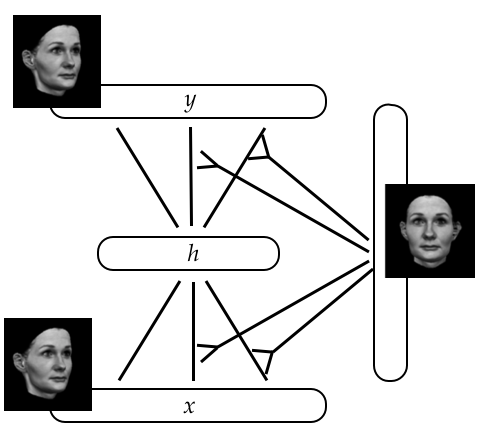
\includegraphics[width=0.25\textwidth]{rae}
}
\subfigure{
 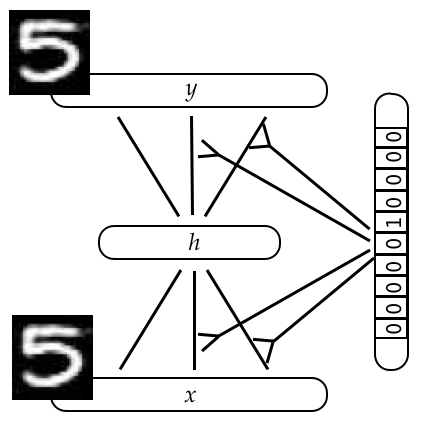
\includegraphics[width=0.22\textwidth]{ccae}
}
\subfigure{
 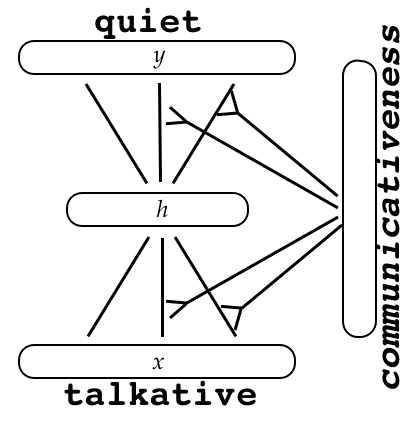
\includegraphics[width=0.21\textwidth]{cccre}
}
\label{f:arch}
\caption{Neural network architectures for RAE, CCRAE, CCCRE.}
\end{figure*}



\subsection{Relational Autoencoders: Background}

Relational autoencoders (RAE), also known as gated autoencoders (GAE),
have been used in computer vision to learn representations of
transformations between images, such as rotation or translation \citep{memisevic:07,memisevic:12,memisevic:13}. RAEs
are a type of {\it gated network}, in which multiplicative connections
between two related inputs are used for prediction or representation
learning. The ``gating'' of one image vector by another allows the feature detectors to concentrate on the correspondences between the related images, rather than being distracted by the differences between untransformed images (Figure~\ref{f:arch}). The key is the use of bilinear connections; there is a weight for every pair of units in the input vector and gate vector. For an overview of RAEs see \citet{memisevic:13,sigaud:15}.
% The connections are known as bilinear because for an image x and its rotated image y, f(y) is a linear function of x, and vice versa.
% The connections are symmetric, but one input is usually considered primary and the other the gate.

We note that despite the terminology, the gates in an RAE perform a somewhat different function than in an LSTM \citep{lstm}. Both network architectures use a nonlinearity to modulate the contents of a product; in an RAE this is an outer (bilinear) product while in an LSTM it is a Hadamard (element-wise) product. However, LSTM gates are memory gates which represent an internal hidden state of the network, while RAE gates are part of the input to the network.

An AE can be defined as follows (we omit bias terms for the sake of simplicity), where $\mathrm{W_e}$ are the encoder weights and $\mathrm{W_d}$ as the decoder weights. In autoencoders it is typical for them to be tied so that $\mathrm{W_d} = \mathrm{W_e}^T$.

\vspace{-5mm}
\begin{equation}
\begin{split}
h & = f(x) = \sigma (\mathrm{W_e}x ) \\
y & = g(h) = \mathrm{W_d}h
\end{split}
\end{equation}
\vspace{-3mm}

For an RAE, we have two inputs $x$ and $z$. Instead of a weight matrix $W$ we have a weight tensor $\overline{\mathrm{W}} \in R^{n_H \times n_X \times n_Z}$.  The RAE is defined as follows.

\vspace{-5mm}
\begin{equation}
\begin{split}
h & = f(x, z) = \sigma ((\overline{\mathrm{W_e}}z)x) \\
y & = g(h, z) = \sigma ((\overline{\mathrm{W_d}}h)z)
\end{split}
\end{equation}
\vspace{-3mm}

\citet{rudy:15} introduce a class-conditional gated autoencoder in which the gate is a one-hot class label, rather than a transformed version of the input image. For example, in the MNIST task the label represents the digit. This is like training an autoencoder per class but with weight sharing across classes. See Figure~\ref{f:arch}(b).

\subsection{Continuous Class-Conditional Relational Encoders}

Our bilinear model is a continuous class-conditional relational encoder (CCCRE). The model architecture is the same as an RAE with untied encoder and decoder weights. However, the training signal differs from a classic RAE in two ways. First, it is not an autoencoder, but simply an encoder, because it is not trained to reproduce the input but rather to transform the input to its antonym. Second, the encoder is class-conditional in the sense of \cite{rudy:15}. In a classic RAE the input and gate are related according to a transformation, but in a class-conditional AE the gate represents the class. Unlike the one-hot gates of \cite{rudy:15}, our gates, representing the semantic domain of the input vector, are real-valued. See Figure~\ref{f:arch}(c).

\section{Experiments}

\subsection{Models}

We compare the CCRE with a number of baseline models. The simplest is cosine similarity in the original vector space. We train a linear model ({\bf Linear}) which maps the input word to its antonym, an Untied Encoder ({\bf UE}) with a bottleneck hidden layer of 150 units, and a shallow feed-forward model ({\bf FF}) with 600 hidden units rather than a bottleneck. To test whether the semantic domain is helpful in learning to negate, each of these models has a {\bf Concat} version in which the input consists of the concatenated input word and gate. {\bf UE-Concat} has 300 hidden units and {\bf FF-Concat} has 600. We did not find using dropout to improve performance in any of our models.

\subsection{Experimental Settings}


We use publicly-available\footnote{\url{https://code.google.com/archive/p/word2vec/}} 300-dimensional embeddings trained on part of the Google News dataset using the skip-gram with negative sampling model of Mikolov et al. (2013).
Antonym training data was obtained from WordNet (hereafter WN), resulting in approximately 20K training pairs.
% We used the antonym relation for WN adjectives, and expanded the initial list of antonym pairs with WN synonyms of each word in the pair. This resulted in approximately 20K (input word, target word) training pairs. 
We exclude any antonym pair with the input word in the test set.

Gates were obtained under three conditions. In the {\bf standard} condition we collect all WN cohyponyms of an input word. If there are fewer than 10 WN cohyponyms, we increase the number to 10 with nearest neighbours from the original vector space. The gate is calculated as the vector centroid of the resulting word list. 

% We did not exclude cohyponyms of the test input words, since the theory is that the network needs these examples to learn the gates / contexts. That is, if 'cold' is in the test set, the model learns how to negate it by learning how to negate other temperature words.

% Neutral context gates were obtained under three conditions. In the {\bf standard} condition we take all WordNet cohyponyms of the adjective
% sense of input word $w$, where cohyponyms include: other lemmas in the synset, children of attribute, synonyms, antonyms, synonyms of the antonyms, similar-tos. If there were fewer than 10 cohyponyms in WordNet, we increased the number to 10 with non-overlapping nearest neighbours from the original vector space. The gate is the centroid of these vectors.

In the {\bf unsupervised} condition we do not use WN to find the semantic neighbourhood, but rather use the ten nearest neighbours from the original vector space. However, the target antonym is still supervised. In the {\bf restricted} condition, we remove all cohyponyms of test input words from the training data. This is to test how important it is to have training examples with similar gates. For example, if {\it cold} is a test word, we remove {\it hot, cold, tepid, cool} etc. from the training data.

We used MSE loss. Hyperparameters were tuned on the GRE development set. The feed forward and CCCRE networks have hidden layers of 600 units, while the UAE has a hidden layer of 150, and 300 for UAE-Concat. Minibatch size was 48 for bilinear networks and 16 for the others. Number of epochs 400 for feed-forward, 200 for bilinear, 300 for UAE, 100 for linear. Optimization adadelta with $\rho = 0.95$.


\subsection{Evaluation}

We evaluted our models with two experiments. Experiment 1 uses the Graduate Record Examination (GRE) questions of \citet{mohammad:13}. The task is, given an input word, to pick the best antonym out of five options. An example from the development set is shown in (\ref{eqn:gre-ex}), where the input word is {\it piquant} and the correct answer is {\it bland}. We restrict the questions to those in which both input and target words are adjectives.

\vspace{-6mm}
\begin{equation}
\begin{split}
\textrm{piquant:\ \ } & \textrm{(a) shocking (b) jovial (c) rigorous} \\
& \textrm{(d) merry (e) {\bf bland}}
\label{eqn:gre-ex}
\end{split}
\end{equation}
\vspace{-4mm}

We evaluate by predicting the antonym for the input word. We measure cosine distance from the predicted vector to each of the five terms in the multiple choice question, and choose the closest term. We report accuracy, i.e. percentage of questions answered correctly.

Experiment 2 evaluates the precision of the models. Recall that our goal was to negate an adjective given its word vector. A natural criterion for success is whether the model returns a good antonym at rank 1, or a few good antonyms at rank 5, rather than returning any particular antonym as required by the GRE task.

We use two datasets: the GRE test set and a set of 99 adjectives and their
antonyms from a dataset collected by Lenci and Benotto
acccording to the guidelines of \citet{walde:13}. For each input word we retrieve the five nearest neighbours of the model prediction and check against a gold standard whether each neighbour is an acceptable antonym.

Gold standard antonyms for an input word $w$ include $w$'s antonyms from the test sets and the WN antonyms of $w$. Following \citet{gorman:05}, to minimise false negatives we improve the coverage of our gold standard by expanding it with antonyms from the online version of Roget's 21st Century Thesaurus, Third
Edition.\footnote{\url{http://thesaurus.com}} We report precision at
ranks 1 and 5.


\section{Results and Discussion}
\begin{table}[t!]
% \centering
% \small
\begin{tabular}{lccc}
 & \multicolumn{3}{c}{\bf Training Condition} \\
\bf Method & \bf Stand. & \bf Unsup. & \bf Restr. \\
\hline
\hline
Random & 0.20 & --- & --- \\
Cosine & 0.50 & --- & --- \\
\hline
Linear & 0.56 & 0.56 & 0.53 \\
Linear-Concat & 0.66 & 0.59 & 0.63 \\
\hline
UE & 0.57 & 0.55 & 0.52 \\
UE-Concat & 0.63 & 0.58 & 0.61 \\
FF & 0.58 & 0.54 & 0.51 \\
FF-Concat & 0.65 & 0.56 & 0.63 \\
\hline
CCCRE & \bf 0.69 & \bf 0.60 & \bf 0.65 \\
\end{tabular} 
\caption{Accuracy on the 367 multiple-choice adjective questions in the GRE test set.}
\label{t:gre}
\end{table}

\begin{table*}[t!]
\centering
\small
\setlength\tabcolsep{1.5pt}
\begin{tabular}{lcc|cc|cc||cc|cc|cc}
& \multicolumn{6}{c||}{\bf GRE} & \multicolumn{6}{c}{\bf Lenci} \\
& \multicolumn{2}{c|}{\bf Stand.} & \multicolumn{2}{c|}{\bf Unsup.} & \multicolumn{2}{c||}{\bf Restr.} & \multicolumn{2}{c|}{\bf Stand.} & \multicolumn{2}{c|}{\bf Unsup.} & \multicolumn{2}{c}{\bf Restr.} \\
\bf Method & \bf P@1 & \bf P@5  & \bf P@1 & \bf P@5  & \bf P@1 & \bf P@5  & \bf P@1 & \bf P@5  & \bf P@1 & \bf P@5  & \bf P@1 & \bf P@5  \\
\hline
\hline
Cosine & 0.05 & 0.07 & --- & --- & --- & --- & 0.13 & 0.10 & --- & --- & --- & --- \\
Linear & 0.36 & 0.29 & 0.34 & 0.29 & 0.32 & 0.28 & 0.29 & 0.25 & 0.30 & 0.24 & 0.29 & 0.23 \\
Linear-Concat & 0.39 & 0.33 & 0.43 & 0.34 & 0.36 & 0.31 & 0.33 & 0.28 & 0.31 & 0.27 & 0.32 & 0.27 \\
\hline
FF & 0.37 & 0.32 & 0.34 & 0.30 & 0.08 & 0.15 & 0.30 & 0.24 & 0.27 & 0.23 & 0.22 & 0.19 \\
FF-Concat & 0.36 & 0.30 & 0.46 & 0.40 & 0.37 & 0.34 & 0.34 &  0.26 & 0.28 & 0.26 & \bf 0.34 & 0.27 \\
UE & 0.38 & 0.33 & 0.36 & 0.32 & 0.37 & 0.31 & 0.28  & 0.22 & 0.27 & 0.23 & 0.23 & 0.20 \\
UE-Concat & 0.38 & 0.33 & 0.43 & 0.38 & 0.27 & 0.31 & 0.33 & 0.28 & 0.34 & 0.27 & 0.28 & 0.25 \\
CCCRE  & \bf 0.66 & \bf 0.49 & \bf 0.52 & \bf 0.42 & \bf 0.52 & \bf 0.38 & \bf 0.39 & \bf 0.32 & \bf 0.46 & \bf 0.32 & \bf 0.34 & \bf 0.30 \\
\end{tabular} 
\caption{Precision at ranks 1 and 5 on the GRE and Lenci datasets.}
\label{t:prec}
\end{table*}

Table~\ref{t:gre} shows the results of Experiment 1. A random baseline results in 0.20 accuracy. The cosine similarity baseline is already fairly strong at 0.50, suggesting that in general about two out of the five choices are closely related to the input word.

Information about the semantic domain clearly provides useful information for this task, because the {\bf Concat} versions of the Linear, UE, and FF models achieve several points higher than the models using only the input word. The linear model achieves a surprisingly high 0.66 accuracy under standard training conditions. The CCCRE model achieves the highest accuracy across all training conditions, and is the only model that beats the linear baseline, suggesting that bilinear connections are useful for antonym prediction.

All the models show a notable loss of accuracy in the {\bf unsupervised} condition,
% , where the gates are built from nearest neighbor vectors rather than WN cohyponyms, 
suggesting that despite the findings of \citet{kruszewski:16}, the alternatives found in the vector neighbourhood are not as accurate for this task. 
% It is possible that their centroid is too close to the input vector to make a useful gate. 
Even in this setting, however, CCCRE achieves a respectable 0.60 accuracy.

In the {\bf restricted} condition, 
% where cohyponyms of the test words are excluded from training, 
all models without the gate vector perform near the cosine baseline, suggesting that in the standard setting they were simply memorising antonyms of semantically similar words. The models with gates retain a higher level of accuracy, suggesting that they are able to generalise across different semantic classes.

Although CCCRE achieves the highest accuracy in Experiment 1, the GRE task does not reflect our intial goal, namely to generate a one-best antonym. CCCRE sometimes fails to predict the specific antonym in the GRE dataset, but still makes a good prediction. For input word {\it doleful}, the model fails to choose the GRE target word {\it merry}, preferring instead {\it sociable}. However, the top three nearest neighbours for the predicted antonym of {\it doleful} are {\it joyful, joyous}, and {\it happy}, all very acceptable antonyms. Experiment 2 measures precision directly.
% This phenomenon is addressed in Experiment 2.

Table~\ref{t:prec} shows the results of Experiment 2. In the standard training condition with supervised gates, CCCRE shows an impressive P@1 of 0.66, i.e. two thirds of the time it is able to produce an antonym of the input word as the nearest neighbour of the prediction. All of the other models score less than 0.4. In the other training conditions CCCRE retains the ability to give a one-best antonym about half the time.

The Lenci dataset is more challenging [TODO: say why]. However, CCCRE still achieves the highest precision.

[TODO: try to fit an example of the top 5 for CCCRE and one other model for an example word or two!]

% [TODO: we expect the network will have the hardest time negating adjs that don't have a good gate, i.e. a well-defined semantic neighbourhood. Look for some examples.]

\section{Related Work}

\citet{widdows:03} introduces a binary negation function for vector
spaces, e.g. {\it suit NOT lawsuit}, which is used for word sense
disambiguation in Information Retrieval. \citet{turney:12,hermann:13}
propose a multi-part vector representation that separates domain and
value, but this does not allow negation of a word in an arbitrary
vector space. \citet{pham:15,nguyen:16,mrksic:16} use ontologies such
as WN or domain-specific ontologies to retrofit embeddings, or learn
embeddings with a secondary objective, pushing synonyms closer
together and antonyms further apart. This improves the overall vector
space and makes it more likely that close words will be synonyms, but
does not provide a way to find antonyms in the
space. \citet{santus:14a,santus:14b,santus:15} perform synonym-antonym
discrimination using an unsupervised measure based on the relative
salience of shared contexts. This type of relation classification does
not make it possible to negate an arbitrary word. \citet{mohammad:13} use a supervised
thesaurus-based method augmented with co-occurrence statistics on the
GRE task (including nouns and verbs). 
% [TODO Maybe de Marneffe on adjective scales.]

[TODO: vision citations for a couple of applications of RAEs]

%  Turney (2008) proposed a supervised algorithm for the identification of several semantic relations, including synonyms and opposites. The algorithm relied on a training set of word pairs with class labels to assign the labels also to a testing set of word pairs. All word pairs were represented as vectors encoding the fruencies of co-occurrence in textual patterns extracted from a large corpus of web pages. He used the seuential minimal optimization (SMO) support vector machine (M) with a radial basis function (RBF) kernel (Platt, 1998) implemented in Weka (Waikato Environment for Knowledge Analysis) (Witten and Frank, 1999). In the discrimination between synonyms and opposites, the system achieved an accuracy of 75% against a majority class baseline of 65.4%. Mohammad et al. (2008) proposed a method for determining the degree of semantic contrast (i.e. how much two contrasting words are semantically close)  based on the use of thesauri categories and corpus statistics. For each target word pair, they used the co-occurrence and the distributional hypothesis to establish the degree of opposition. Their algorithm achieved an F-score of 0.7, against a random  baseline of 0.2. Mohammad et al. (2013) used an analogical method based on a given set of contrasting words to identify and classify different kinds of opposites by hypothesizing that for every opposing pair of words, A and B, there is at least another opposing pair, C and D, such that A is similar to C and B is similar to D. For example, for the pair
% . Given the existence of contrast, they calculated its degree relying on the
% co-occurrence
%  hypothesis. Their approach outperformed other state-of-the-art measures

\section{Conclusion}

We have shown that a neutral context vector, representing the set of alternatives, improves antonym prediction in linear and non-linear models, and that the multiplicative connections in a bilinear model are effective at learning to negate adjectives. In the broader context of modelling closed-class function words, it is perhaps not too farfetched to imagine that a specialised network with multiplicative connections might be necessary to model these kinds of words.

Our implementation is a simple one, using a full tensor for the bilinear layer, and takes several hours to train on a GPU. Future work will exploit the many options for reducing the number of parameters to be learned \citep{alain:13} and address negation of nouns and verbs, where negation is more likely to involve a probability distribution over alternatives---e.g. {\it didn't run} might mean {\it walk} or {\it amble}---rather than predicting a single best antonym.

\bibliographystyle{myplainnat}
\bibliography{eacl2017}
% \bibliographystyle{eacl2017}


\end{document}
